\section{Introduction}

\subsection{Motivation}


Fluid is everywhere, from the air we breath, the water we drink to the wind flow around the air craft. Computational fluid dynamics (CFD) is a science that \cite{thelbmbible}, with the help of digital computers, produces quantitative predictions of fluid-flow phenomena based on the conservation laws (conservation of mass, momentum, and energy) governing fluid motion. Computational fluid dynamics has been applied to many aspects of our society, including wind simulation for aircraft, fire simulation in environment engineering and even the airflow around face masks simulation during the COVID-19. On the commercial side, the market size of CFD industry in 2016 is over 20 times larger than 2001; see Fig.~\ref{fig:cfd_market}. In 2019, The Worldwide Computational Fluid Dynamics (CFD) market size was USD 1703.5 million and it is expected to reach USD 3200.3 million by the end of 2026\cite{market_cfd}.\\

\begin{figure}[htbp]
    \centering
    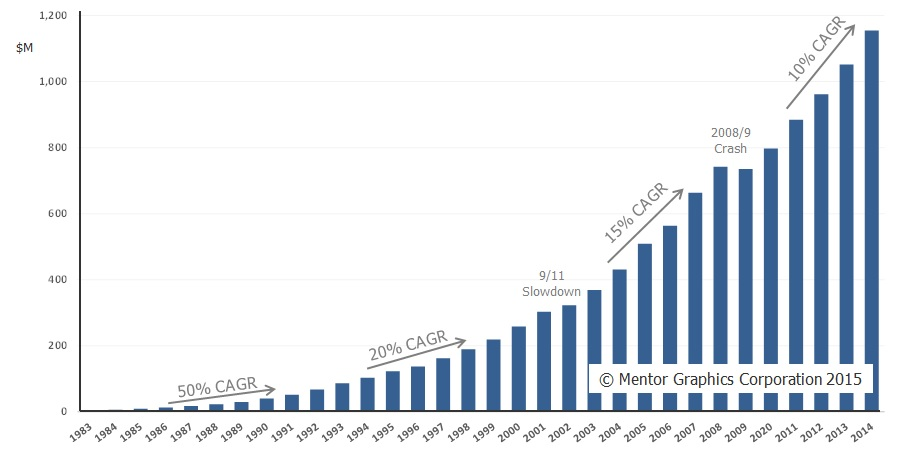
\includegraphics[width=1\textwidth]{figures/CFD_market.jpg}
    \caption{The global market size of CFD industry. From the early 1983, the market size has been increasing significantly reaching over 1200 million dollars by 2014. The trend has been predicted to continue. (Image from \cite{market_cfd})}
    \label{fig:cfd_market}
\end{figure}

As the definition says, CFD highly rely on computers, especially high-performance computers (HPC). Indeed, quite an objective part of HPC resource also goes to fluid dynamics simulation; see \ref{fig:break_down}. However, the simulation is becoming more demanding, and the CFD poses new challenges to HPC every year. For example, Formula 1 racing teams give high priority to aerodynamics simulation and they always want to run as much simulation as possible within a short period of time. If they want to beat the other F-1 teams in the aerodynamics, they need to run simulation faster in a more powerful supercomputer while the Fédération Internationale de l'Automobile (FIA) start to limit the power consumption of the CFD simulation \cite{formula1} of F-1 teams. Engineers like them from all areas face the similar challenge and they need to figure out a feasible way.

\begin{figure}[!tb]
    \centering
    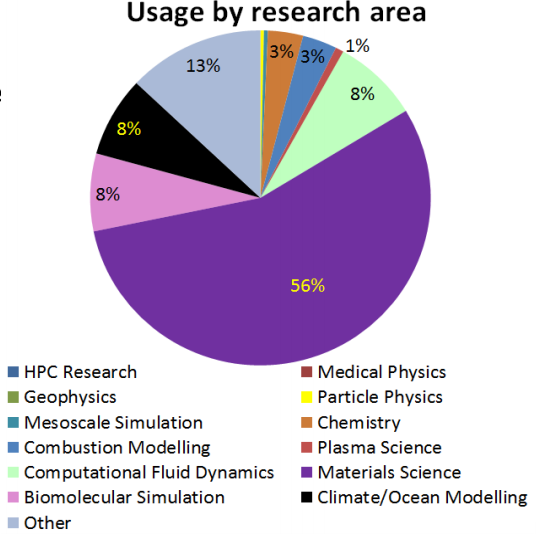
\includegraphics[width=0.7\textwidth]{figures/break_down.png}
    \caption{The HPC usage in ARCHER by research area in July 2016. Computational fluid dynamics related areas (including mesoscale simulation, combustion modeling and CFD) took over 10\% of the total use. (Image from \cite{archer_use}))}
    \label{fig:break_down}
\end{figure}


% \begin{figure}[!tb]
%   \centering
%       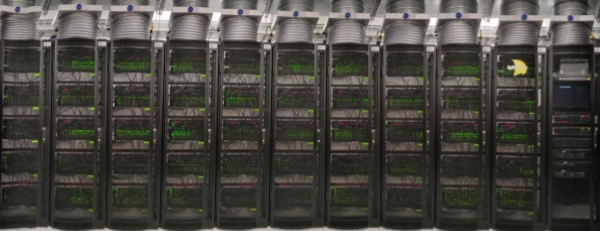
\includegraphics[width=0.7\textwidth]{figures/cluster.png}
%       \caption{The 500,000-core SpiNNaker \textit{102} machine at the University of Manchester (image from \cite{spinn-core}).}
%       \label{fig:cluster}
% \end{figure}


% Nowadays, the amount of data has grown increasing large, traditional computer architectures do not scale as the Moore's law. While parallelism is regarded as an option to keep the scaling, the SpiNNaker hardware was designed to be massively distributed and parallel. Thus the SpiNNaker hardware has the potential to be used as a parallel computing solution. As opposite to the traditional hardware, SpiNNaker has the following hardware features:

% \begin{itemize}
% \item \textbf{Manycore architecture}: though modern CPUs start to have multiple cores to gain some parallelism, the number of cores in a CPU is usually less than 10. On the opposite, a type Spinn-5 SpiNNaker board has 48 chips, which contains hundreds of ARM cores \cite{5th-summit}. Though there are more cores, because of the medium-performance (only 200MHz) ARM968 cores, the energy consumption stays relatively low.

% \item \textbf{Communication model}: the SpiNNaker cores communicate by sending message via UDP/IP \cite{ws6} and UDP/IP do not guarantee the delivery. Though it is the developers' responsibility to make sure the correctness, the developers do not need to worry about the dead-lock. It is designed as so because in a real human brain a neuron does not get any an acknowledgement when the communication is done \cite{spinnaker}.

% \item \textbf{Communication throughput}: extra performance might be gain from the reduce of the message size and more message can be process in the same amount of time\cite{furber2012overview}. Their link can transfer up to 31.25M byte/s, which means the links can handle 3M packets per second \cite{ws6}.\\
% \end{itemize}

Meanwhile, some neuromorphic hardware has been actively developed during the same period of time. SpiNNaker (Spiking Neural Network Architecture) is one of them. SpiNNaker  \cite{thespinnbible} is an approach to build a machine that is based to some degree on what is understood about the principles of operation of the human brain. It has the following hardware features:
\begin{itemize} 
\item \textbf{Massively parallel:} A single type Spinn-5 SpiNNaker board has 48 SpiNNaker chips. Each SpiNNaker chip has 18 ARM cores, which means the board has up to $48 \times 18 = 864$ cores. Each core has the ability to simulate at least 256 neurons. The SpiNNaker clusters are build with cabinets of boards. The SpiNNaker can bring massive parallelism.

\item \textbf{Low energy-consumption:} Opposite to the conventional HPC which are usually build up with energy-hungry cores running in GHz, the SpiNNaker only need 1 watt per chip.

\item \textbf{Communication model:} The communication model we primarily used is multicast. The cores can pass messages to multiple destinations by a single send.
\end{itemize}


In a word, the SpiNNaker has the full features as a supercomputer and it could provide new opportunities for parallel software engineers and CFD engineers. However, there is not much scientific applications developed on SpiNNaker, especially CFD applications. In this project, we will explore the potential of using SpiNNaker for CFD simulation and trying to achieve a good performance in terms of speed.\\
 
% On the other side, Computational fluid dynamics (CFD) is a science that, with the help of digital computers, produces quantitative predictions of fluid-flow phenomena based on the conservation laws (conservation of mass, momentum, and energy) governing fluid motion \cite{thelbmbible}. It help us to to solve real-world engineering problems, including aerospace engineering, meteorology, etc. However, CFD algorithm usually involve heavy computation. To get the simulation result in affordable time, scientists and engineers need to accelerate the simulation. Therefore, parallel computers including some supercomputers are heavily used for CFD simulation.\\

Lattice Boltzmann method (referred to as LBM in the rest of this report) is a mesoscopic CFD model which is recognized\cite{lbmmbook} as: (1) easy to apply to complex domain (2) No need to solve the Laplace equation (3) More importantly for this project, being naturally adapted to parallel processing due to the locality and explicit nature of the method. Due to its (3) nature, many parallel techniques are applied to accelerate the LBM simulation, including MPI\cite{he1999three}, OpenMP\cite{massaioli2002achieving} and GPGPU\cite{rogers1990upwind}, etc. \\

As we discussed above, the SpiNNaker has the ability to compute in massively parallel. Thus, there is a perfect match between the SpiNNaker and the lattice Boltzmann method. It is promising that we can get high performance and scalability in term of speed with SpiNNaker's low energy-consumption cores on the LBM simulation tasks, which is also the motivation behind this project.  \\




\subsection{Objectives} \label{sec:Obj}

Firstly, we can define our objective of this projects as follow:\\

\begin{quote}
Implementing a basic lattice Boltzmann method simulation on the SpiNNaker platform; and investigate its  performance and scalability in terms of speed. \\
\end{quote}

% KS: In point one there are two separate points which should be discussed seaparately. First, there is the implementation of the algirthm. Second, there
% is the use of a standard test problem to check that the implementation is
% working correctly. A wide range of test problems could be used.

% KS: There needs to be more here. It's not just a question of implementation. There
% needs to be some critical evaluation of ease-of-use, performance, and so on. 
% to add to KS. you need to discuss how your going to compare. speed, scale? energy? accuracy?

Firstly, we need to implement a standard lattice Boltzmann method on CPU as a reference, which can be more easily to understand and porting the algorithm; and we can also further evaluate the correctness, accuracy and compare the performance with this CPU implementation.\\

Secondly, we need to choose a pre-defined problem as the test problem from a wide range of the problems. As the test problem, it need to be generic and easy to check the correctness. To choose it, we take LBM model and the boundary condition into consideration, and, finally, a two dimensions and nine vectors (D2Q9) model with a periodic condition problem described by Minion and Brown \cite{minion1997performance} was chosen. It is generic -- D2Q9 model is widely used, and easy to check the correctness -- with the mentioned initial condition, there will be a turbulence in a fix step and we can check it.\\

Then, we focus on the design and implementation of the LBM on the SpiNNaker. For each step of the LBM, we need to carefully design and implement, especially for the communication in SpiNNaker with the SpiNNaker software stack \cite{software_spinn}. This is also the main part of this project.\\

Finally, after implementing the simulation on SpiNNaker, we will to evaluate correctness and accuracy the simulation result by compare the numbers in quantitatively. After we confirm the correctness, them some experiment would be focus on optimization the communication and bench mark the result with the standard CPU implementation on speed-ups and scalability.\\

\subsection{Project Overview}

The work of this project are threefold:\\

 \textbf{A basic lattice Boltzmann implementation on CPU}: we firstly built a standard serial implementation of a pre-defined lattice Boltzmann scenario described by Minion and Brown \cite{minion1997performance}; see Subsection \ref{sec:ip}. \\

 \textbf{A basic lattice Boltzmann implementation on SpiNNaker:} after we implemented the simulation on CPU, we used the CPU implementation as a reference to implement the same simulation on SpiNNaker platform with some of the SpiNNaker software development kit; see Section \ref{sec:dai}\\

\textbf{An investigation on the speed performance and scalability}: we demonstrate that lattice Boltzmann on SpiNNaker platform offers better speed performance in larger scale when compared to CPU and it also has a good scalability on weak-scaling. We bench-marked two implementations of the lattice Boltzmann method scenario: the first one is the standard implementation of on a normal Intel CPU and second one is a implementation on SpiNNaker mentioned above. The observation shows that lattice Boltzmann program can gain  $277.192 / 60.01 = 4.61$ speed-up in terms of speed over a certain scale; see Section \ref{sec:perfe}.



